\documentclass{article}
\usepackage[margin=1in]{geometry}
\usepackage{graphicx}
\usepackage{xcolor}
\usepackage{float}
\usepackage{amsmath}
\usepackage{cite}
\usepackage{hyperref}
\usepackage{indentfirst}
\graphicspath{{..} {./images}}

\definecolor{navy-blue}{rgb}{0.22,0.38,0.71}

\renewcommand{\contentsname}{\vspace*{-2\baselineskip}}

\hypersetup{
	colorlinks,
	linkcolor=black,
	urlcolor=blue,
	citecolor=black
}
  		
\begin{document}
\begin{titlepage}
	\centering
	{\huge Lab 7 - Digital Modulation: Frame Synchronization}\\[0.25 in]
	
\includegraphics[width=0.6\textwidth]{ua_logo.png}\\[0.25 in]
	{\large \textbf{ECE 531 - Software Defined Radio\\[0.25 in]
	April 18, 2025\\[0.25 in]}}
	{\large Owen Sowatzke, osowatzke@arizona.edu\\[0.05 in]
	Department of Electrical \& Computer Engineering\\[0.05 in]
	University of Arizona, Tucson, AZ 85721\\[0.5 in]}
	\hypersetup{linkcolor=navy-blue}
	\noindent\hrulefill
	\tableofcontents
	\noindent\hrulefill
\end{titlepage}

% \setlength{\parindent}{0pt}

\section{Introduction}
%Introduction to the laboratory experiment, including a brief description of the objectives and goals.

In this lab, we perform frame synchronization on data generated in MATLAB. Correct frame alignment is critical for correctly recovering the transmitted data. To detect the start of a packet, we specifically cross-correlate our received data with a known preamble. As part of our work in this lab, we learn how to perform cross-correlation with MATLAB's \texttt{filter} command. We also explore performance tradeoffs between the \texttt{xcorr} and \texttt{filter} commands. Finally, we implement a custom frame synchronization routine and evaluate its detection probabilities and packet error rates. The work that follows is divided into two sections. One provides the procedures for each of our experiments, and the other presents the results.

\section{Procedure}
% Detailed explanation of the laboratory experiment, including the design, implementation, and testing of the system.

In this section, we provide the procedure for each of our experiments. We perform frame synchronization (i.e. detect the start of frames) that are consistent with the structure shown Figure \ref{fig::frame_structure}.

\begin{figure}[H]
	\centerline{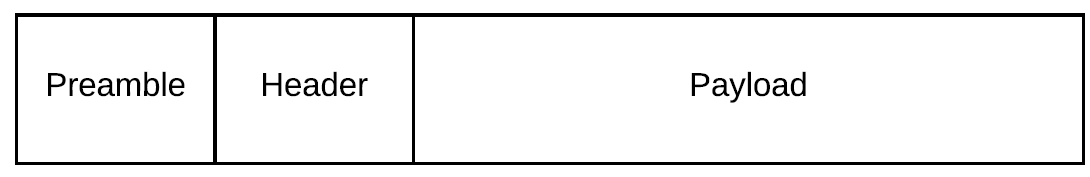
\includegraphics[width=0.6\textwidth]{frame_structure.png}}
	\caption{Frame Structure of a Wireless Packet}
	\label{fig::frame_structure}
\end{figure}

\noindent The preamble in our frames is known by both the transmitter and receiver. For our experiments, we specifically use concatenated barker sequences. Because the preamble is known by the receiver, we can cross-correlate our received data with the preamble using the following equation:

\begin{equation}
	C_{xy}(k) = \sum_{m}{x^*(m)y_n(m+k)}
\end{equation}

\noindent Then, we can use the peak of the cross-correlation output to determine the delay of the frame. In the lab, we execute the provided \texttt{lab7part1.m} script to perform frame synchronization. This script uses MATLAB's \texttt{xcorr} command to perform the cross-correlation. The \texttt{xcorr} command produces an output that is $2L_r - 1$ samples long, where $L_r$ is the length of the longest sequence. The center of its output corresponds to zero delay. Therefore, we can estimate the delay of our frame ($\hat{p}$) as follows:

\begin{equation}
	\hat{p} = \underset{k}{\text{argmax}}\ C_{xy}(k) - L_r
\end{equation}

\noindent For our first experiment, we replace the \texttt{xcorr} command in \texttt{lab7part1.m} with the \texttt{filter} command and validate the correctness of our implementation. Next, for different preamble lengths, we compare the execution time of our updated routine to the original execution time. Then, we use the template given in \texttt{lab7part2.m} and the example given in \texttt{lab7part1.m} to implement a custom frame synchronization routine. Finally, we evaluate the performance of our custom frame synchronization routine across SNRs in range [0,10] dB. As part of our performance analysis, we generate plots of the detection probability and packet error rate.
 
\section{Results}
% Results and discussion of the laboratory experiment, including captured outputs, observations, and responses to laboratory questions.

In this section, we provide the results for each of our experiments. In our experiments, we specifically implement cross-correlation with MATLAB's \texttt{filter} function and compare its execution time to the \texttt{xcorr} command. Then, we create a custom frame synchronization routine and evaluate its detection probabilities and packet error rates for different SNRs.

In Figure \ref{fig::xcorr_preamble_detect}, we show the cross-correlation outputs generated by \texttt{lab7part1.m}, which uses MATLAB's \texttt{xcorr} command to perform the correlation. Note that our cross-correlation output includes a large leading zero region. This occurs because we are zero-padding the preamble and time-advancing it for each point left of the center. For each of these additional samples, we get an element-wise multiplication with zeros followed by a sum of zeros.

\begin{figure}[H]
	\centerline{\fbox{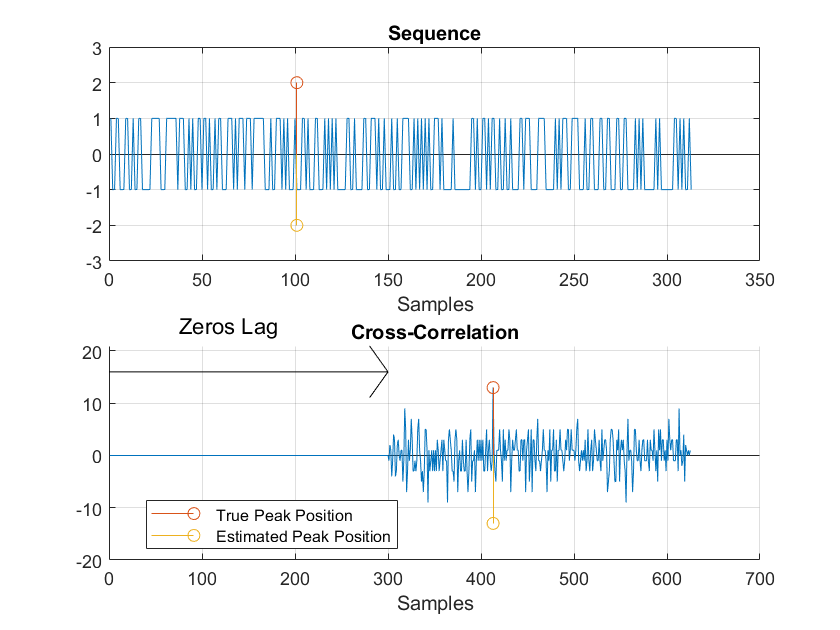
\includegraphics[width=0.5\textwidth]{xcorr_preamble_detect.png}}}
	\caption{Detecting Start of Preamble with \texttt{xcorr} Command}
	\label{fig::xcorr_preamble_detect}
\end{figure}

The \texttt{xcorr} function uses an FFT to perform a correlation, which can be slow for short sequences. As a result, we replace the \texttt{xcorr} function with a \texttt{filter} function. The filter function implements convolution of the following form:

\begin{equation}
	z(k) = \sum_{m}{y_n(m)h(k - m)}
\end{equation}

\noindent We can perform cross-correlation with convolution by letting $h(k) = x^*(-k)$. In other words, we can use a flipped and conjugated version of our preamble as a matched filter. Doing so, we get the results shown in Figure \ref{fig::filter_preamble_detect}.

\begin{figure}[H]
	\centerline{\fbox{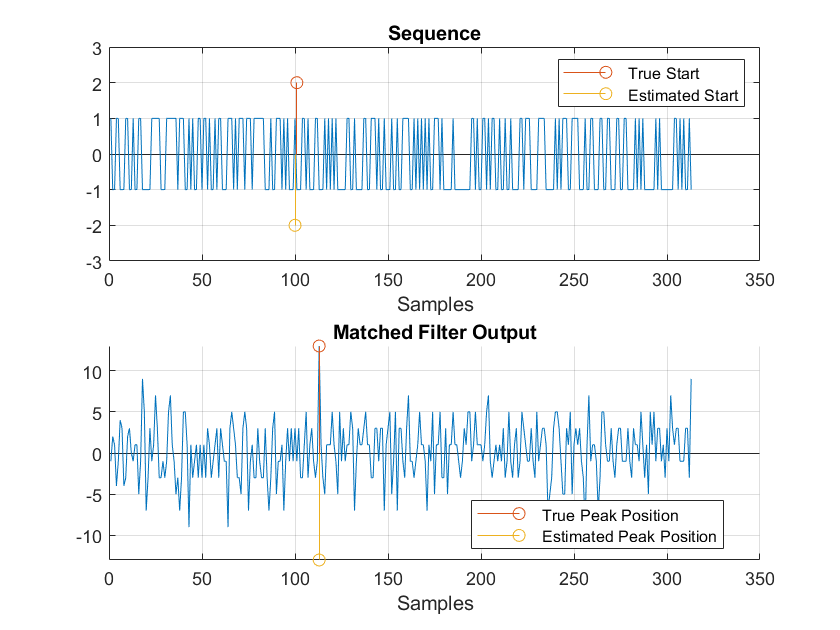
\includegraphics[width=0.5\textwidth]{filter_preamble_detect.png}}}
	\caption{Detecting Start of Preamble with \texttt{filter} Command}
	\label{fig::filter_preamble_detect}
\end{figure}

\noindent Note that the peak from our \texttt{filter} output occurs in a different location. However, we get the same delay estimate as the \texttt{xcorr} function if we account for the offsets in our output. The filter output specifically peaks when the last sample of our preamble is input to the filter. If our preamble length is given by $L_p$, we can estimate the delay from our filter output $z(k)$ as follows:

\begin{equation}
	\hat{p} = \underset{k}{\text{argmax}}\ z(k) - L_p
\end{equation}

\noindent In Figure \ref{fig::execution_time}, we compare the execution time of the \texttt{xcorr} and \texttt{filter} commands for sequence lengths in range [10, 2000]. For each sequence length, we perform 1000 Monte Carlo runs to estimate the average runtime.
 
\begin{figure}[H]
	\centerline{\fbox{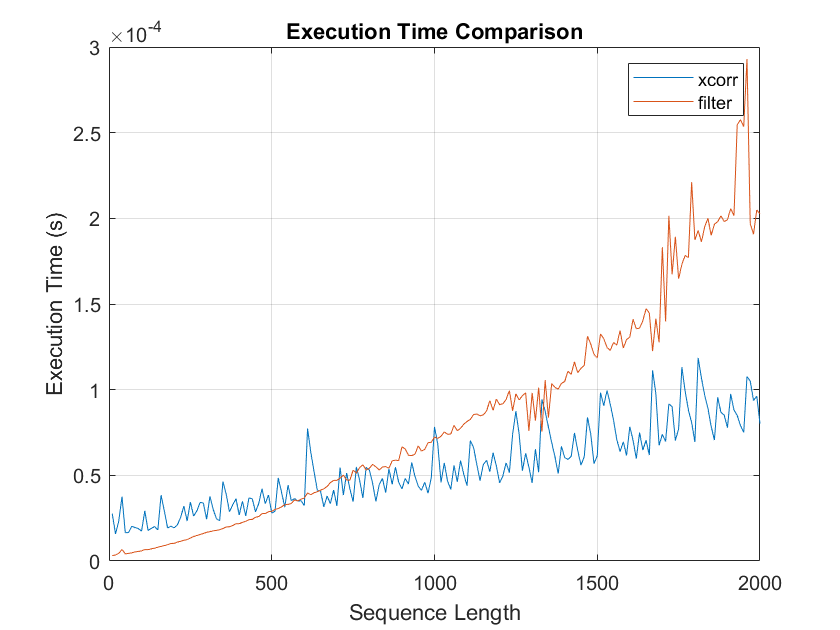
\includegraphics[width=0.5\textwidth]{execution_time.png}}}
	\caption{Comparison of \texttt{xcorr} and \texttt{filter} Execution Time}
	\label{fig::execution_time}
\end{figure}

\noindent Examining the execution times of both routines, we see that the \texttt{filter} command is faster for small sequence lengths ($< 500$), while the \texttt{xcorr} routine is faster for large filter lengths ($> 500$). For small filter lengths, time-domain filtering ( i.e. \texttt{filter}) is faster than frequency-domain filtering (i.e. \texttt{xcorr}) because it avoids the overhead of doing FFTs/IFFTs. However, as the filter length increases, the complexity of the time-domain filter increases faster than the complexity of the frequency-domain filter. In Figure \ref{fig::speedup}, we compute the speedup of the \texttt{filter} routine by dividing the average execution time of the \texttt{filter} command by the average execution time of the \texttt{xcorr} command. Examining the figure, we see that the \texttt{filter} command is approximately 8x faster for sequence lengths of 10, but is roughly half as fast for sequence lengths of 2000. The sequence lengths we use for the rest of the lab are small ($<< 500$), so we use the \texttt{filter} command.  

\begin{figure}[H]
	\centerline{\fbox{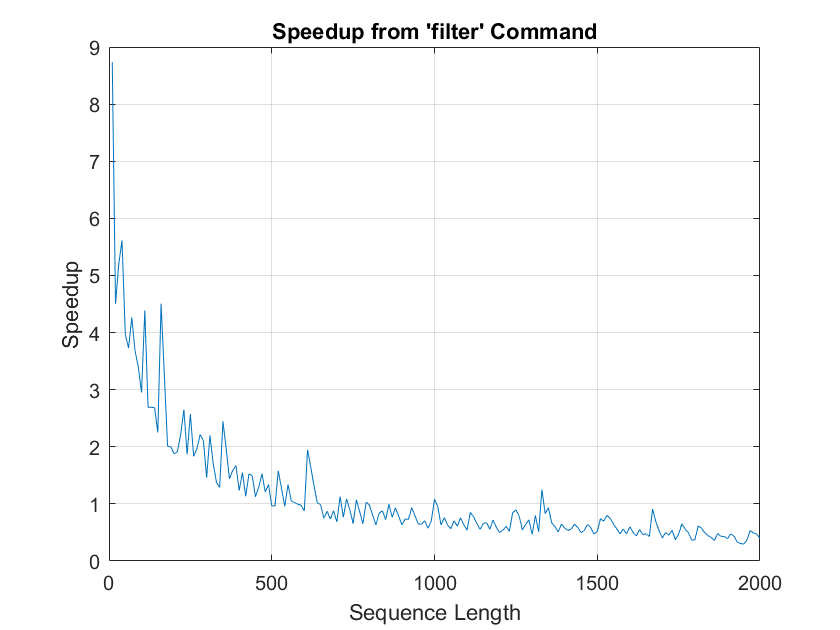
\includegraphics[width=0.5\textwidth]{speedup.png}}}
	\caption{Speedup from \texttt{filter} Command}
	\label{fig::speedup}
\end{figure}

Next, we implement a custom frame synchronizer in MATLAB. Our frame synchronizer uses the \texttt{filter} command to cross-correlate the received data with the preamble. It then normalizes the cross-correlation output to a range between 0 and 1 using the following formula:

\begin{equation}
	r(k) = \frac{C_{xy}(k)}{\sqrt{\sum_m{|x(m)|^2}}\sqrt{\sum_m{|y(m)|^2}}}
\end{equation}

\noindent This formula closely resembles the normalized correlation coefficient, which is described in \cite{pearson_correlation_coefficient}. The normalization function scales the input data, so it has a unit average power and divides the resulting correlation output by the code length. This makes the peak of the correlation output 1 instead of the preamble length. Whenever the magnitude of the normalized correlation output exceeds a threshold ($|r(k)| > T$), we mark the sample as the start of a preamble. For a more efficient hardware implementation, we can also implement the comparison as follows:

\begin{equation}
	|C_{xy}(k)|^2 > T^2\left(\sum_m{|x(m)|^2}\right)\left(\sum_m{|y(m)|^2}\right) = \alpha\sum_m{|x(m)|^2}
\end{equation}

\noindent Using our custom routine, we generate a receiver operating characteristics (ROC) curve, which is included in Figure \ref{fig::roc_curve}.

\begin{figure}[H]
	\centerline{\fbox{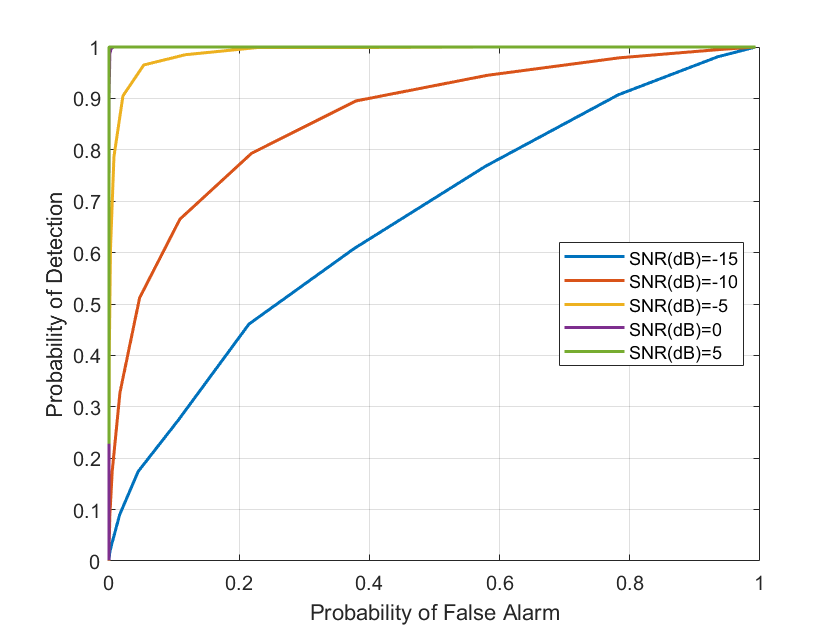
\includegraphics[width=0.5\textwidth]{roc_curve.png}}}
	\caption{Receiver Operating Characteristics}
	\label{fig::roc_curve}
\end{figure}

\noindent For a given SNR, we see that increasing our threshold decreases the probability of false alarm and the probability of detection. Similarly, decreasing our threshold increases the probability of false alarm and the probability of detection. Any threshold we choose will result in points at specific locations on the ROC curve. As a result, when we choose our threshold, we have to trade off probability of detection and probability of false alarm.

We test our frame synchronization routine over SNRs in range [0, 10] dB. To evaluate its performance, we measure the detection probability and packet error rate. The detection probability is the probability we correctly detect the start of the packet, and the packet error rate is the probability that any bit in our packet contains an error. For our analysis, we also consider missed detections as packet errors. For our initial analysis, we consider the peak of the cross-correlator output as the start of a frame. In this configuration, we achieve the best possible performance. Our results are included in Figures \ref{fig::detection_probability_peak} and \ref{fig::per_peak}.

\begin{figure}[H]
	\centerline{\fbox{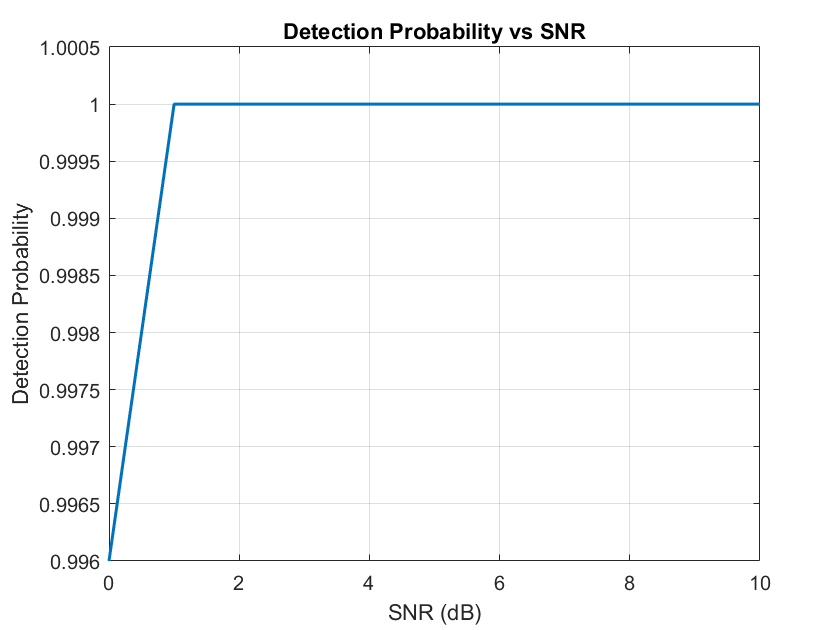
\includegraphics[width=0.5\textwidth]{detection_probability_peak.png}}}
	\caption{Best Case Detection Probability}
	\label{fig::detection_probability_peak}
\end{figure}

\begin{figure}[H]
	\centerline{\fbox{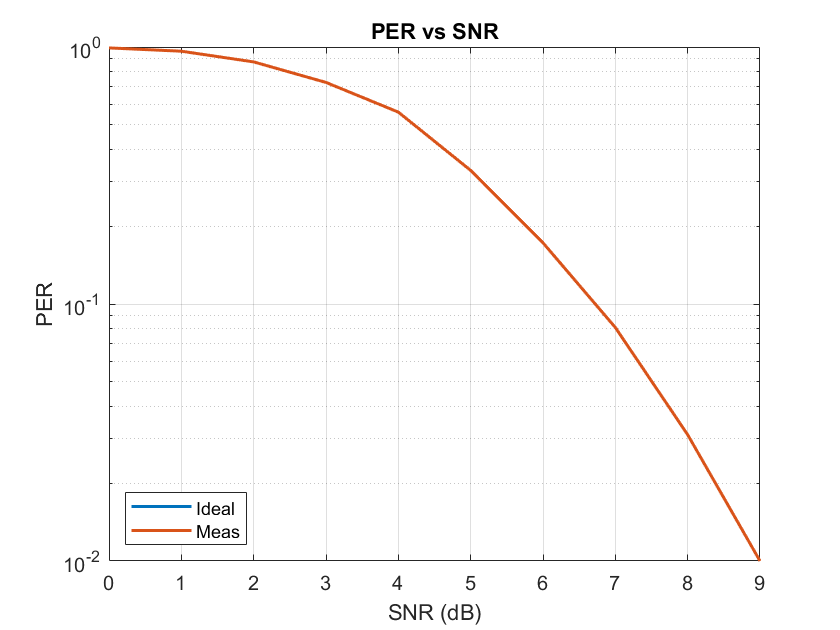
\includegraphics[width=0.5\textwidth]{per_peak.png}}}
	\caption{Best Case Packet Error Rate}
	\label{fig::per_peak}
\end{figure}

\noindent Examining the figures, we see that the detection probability is nearly 1 in all cases. Our preamble is 26 symbols long and provides a coherent gain of $10\log_{10}(26) = 14.15 \text{dB}$. This allows us to maintain high detection probabilities even at low SNR. The packet error rate is high, approaching 1 for SNRs of 0dB. This occurs because the payload bits do not get any coherent gain from the preamble. Additionally, all the bits in the packet must be right for us to correctly decode a packet. As a result, we can express the packet error rate as follows:

\begin{equation*}
	\text{PER} = 1 - (1 - \text{BER})^N
\end{equation*}

\noindent Examining the equation, we see that the PER degrades as the packet length increases.

So far, we have only considered the peak locations in our frame synchronization. Next, we consider the effects of adding a threshold, which is necessary for preventing false alarms. For this analysis, we consider the first point in the frame that exceeds the threshold as the start of a packet. This is consistent with the algorithm presented in MATLAB's \texttt{comm.PreambleDetector}. Our results are included in Figures \ref{fig::detection_probability_first} and \ref{fig::per_first}.

\begin{figure}[H]
	\centerline{\fbox{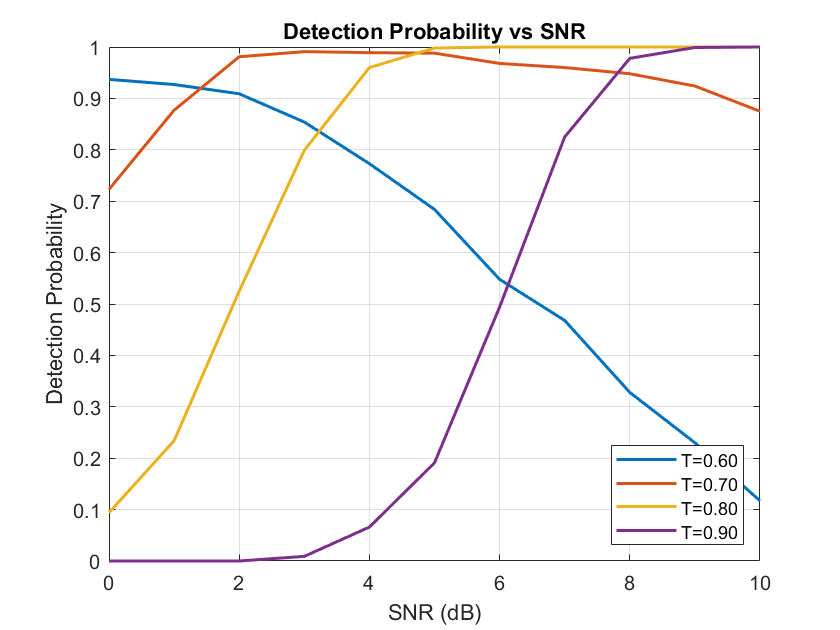
\includegraphics[width=0.5\textwidth]{detection_probability_first.png}}}
	\caption{Detection Probability Using First Sample That Exceeds Threshold}
	\label{fig::detection_probability_first}
\end{figure}

\begin{figure}[H]
	\centerline{\fbox{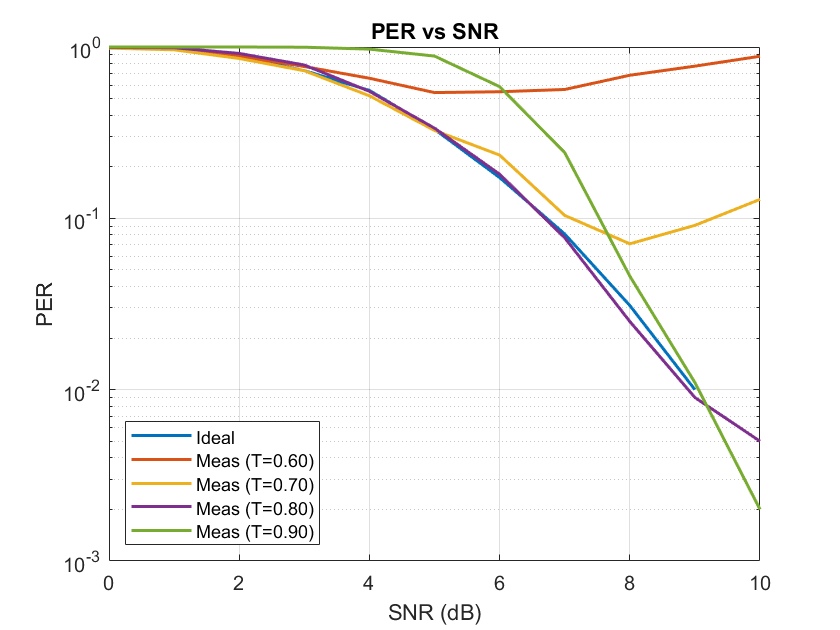
\includegraphics[width=0.5\textwidth]{per_first.png}}}
	\caption{Packet Error Rate Using First Sample That Exceeds Threshold}
	\label{fig::per_first}
\end{figure}

\noindent Comparing our detection probability to the results in Figure \ref{fig::detection_probability_peak}, we see that lower thresholds result in higher detection probabilities at low SNR. However, as our SNR increases, our probability of detection falls. This is because the sidelobes of our cross-correlation output exceed our threshold and are selected as the start of the frame. The auto-correlation of our preamble before and after normalization is shown in Figure \ref{fig::auto_corr_preamble}.

\begin{figure}[H]
	\centerline{\fbox{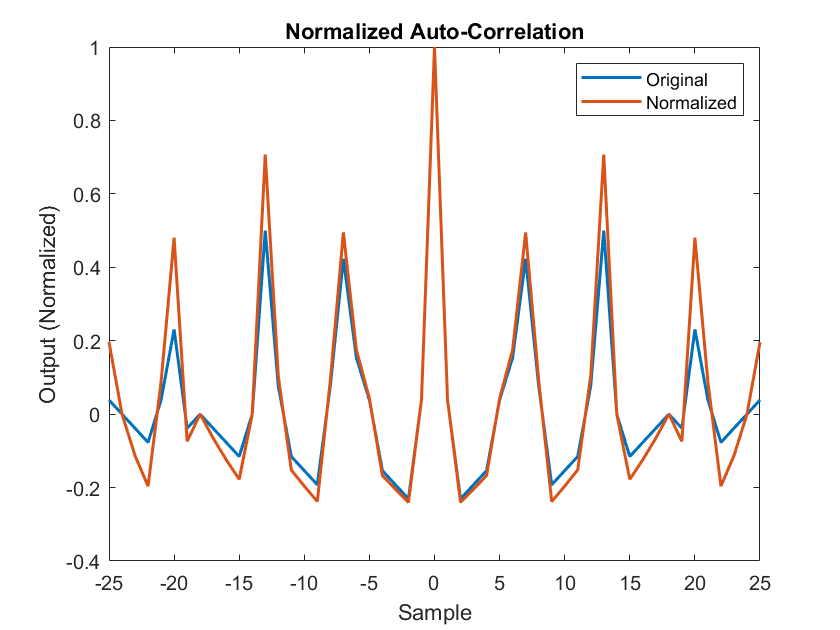
\includegraphics[width=0.5\textwidth]{auto_corr_preamble.png}}}
	\caption{Auto-Correlation of Preamble}
	\label{fig::auto_corr_preamble}
\end{figure}

\noindent Examining the correlation output, we see that that normalizing the response increases the sidelobe amplitude. This occurs because the average power of our input is lower at the start of the correlation because there are fewer non-zero samples being input to the correlator. This problem gets worse as the SNR increases because the noise samples have less power. However, for sufficiently high thresholds, we should be able to mitigate this issue. In Figure \ref{fig::per_first}, for example, we see that setting the threshold to 0.8 results in an almost ideal packet error rate. However, we also note that our low SNR detection probability degrades.

	In addition to increasing the threshold, another solution that I came up with examines a full preamble length of samples when the threshold is exceeded. It specifically finds which samples results in the largest peak and marks the preamble position accordingly. This extra logic helps the frame synchronizer ignore sidelobes in the cross correlation output when operating with a lower threshold. In other words, we can reduce our threshold to improve low SNR performance, while simultaneously maintaining high SNR performance. The updated algorithm results are shown in Figures \ref{fig::detection_probability_mod} and \ref{fig::per_mod}.
	
\begin{figure}[H]
	\centerline{\fbox{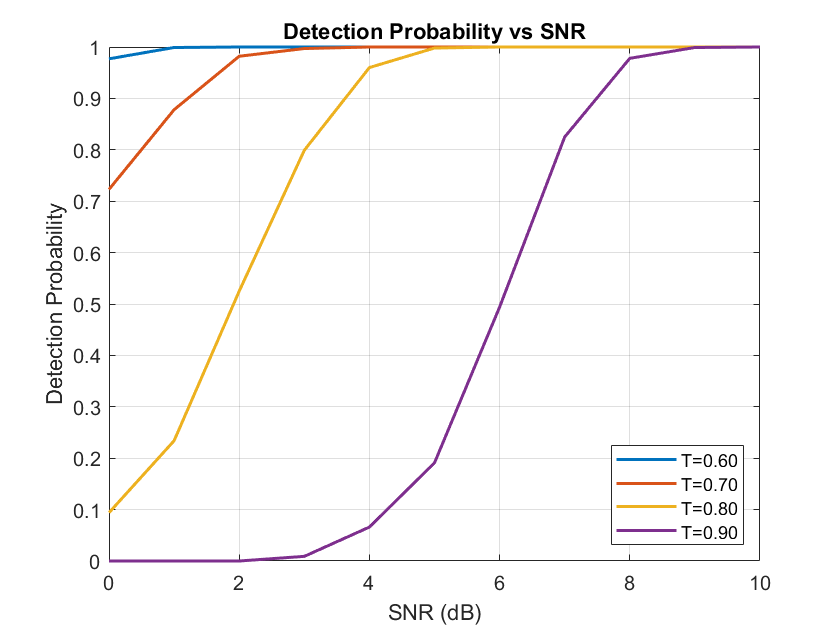
\includegraphics[width=0.5\textwidth]{detection_probability_mod.png}}}
	\caption{Detection Probability Using Modified Algorithm}
	\label{fig::detection_probability_mod}
\end{figure}

\begin{figure}[H]
	\centerline{\fbox{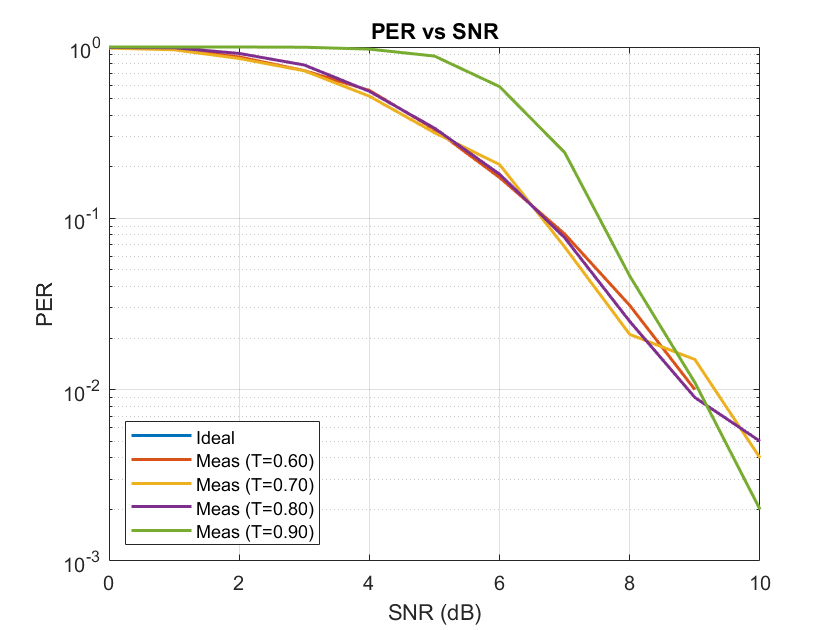
\includegraphics[width=0.5\textwidth]{per_mod.png}}}
	\caption{Packet Error Rate Using Modified Algorithm}
	\label{fig::per_mod}
\end{figure}

\noindent Compared to our prior results in Figures \ref{fig::detection_probability_first} and \ref{fig::per_first}, we see that the modified algorithm maintains low threshold performance even at higher SNRs. In contrast to our previous results, a threshold of 0.6 now appears best for performance. Note that this algorithm is designed specifically to improve performance for large swings in the input power. If we had back-to-back frames of data, the original normalization algorithm would be sufficient. Finally if desired, we can also offshore our normalization and/or thresholding computations. MATLAB's \texttt{comm.PreambleDetector}, for example, does not include normalization. Therefore, we could hypothetically design a better normalization algorithm, which would maintain the same scaling during the cross-correlation of frame data. This in turn would allow us to have larger peak to sidelobe ratios, which finally would improve the detection and/or the false alarm probability.

\section{Conclusion}
% Conclusions to the overall lab that discuss meaningful lessons learned and other takeaways from the assignment. (Important)

In this lab, we performed frame synchronization on data generated in MATLAB. To do this, we cross-correlated our received data with the preamble. The peak of our cross-correlation output then helped us correctly locate the frame. In MATLAB, we performed the cross-correlation in two separate ways: \texttt{xcorr} and \texttt{filter}. For the \texttt{filter} commmand, we used a flipped and conjugated version of the preamble as our FIR filter. To determine delays from the the \texttt{xcorr} command, we had to subtract $L_r$ (length of the longest sequence) from our peak index. Similarly for the \texttt{filter} command, we had to subtract $L_p$ (preamble length) from our peak index.

We also compared the runtimes of both routines. The \texttt{xcorr} command used an FFT to compute the correlation, while the \text{filter} command performed correlation in the time domain. As a result, we found that the \texttt{xcorr} command took longer to run for small preamble lengths ($ < 500$) , while the \texttt{filter} command took longer to run for large preamble lengths ($ > 500$). All the preamble lengths used in the lab were very short ($ << 500$). Therefore, we used the \texttt{filter} command instead of the \texttt{xcorr} command for the remainder of the lab.

Next, we created a custom frame synchronizer in MATLAB. Our routine closely resembled MATLAB's \texttt{comm.PreambleDetector}. It specifically applied a threshold to the cross-correlation output to determine when a frame was present. It also performed normalization to simplify the thresholding for different signal strengths. The normalization made both inputs unit power and accounted for the maximum coherent gain (preamble length gain) during cross-correlation. Using our routine, we generated an ROC curve. The ROC curve allowed us to perform tradeoffs between the detection and false alarm probabilities.

Then, we evaluated the performance of our frame synchronizer by examining detection probabilities and packet error rates for SNRs in range [0, 10] dB. We started our analysis by using the peak index of the cross-correlation output. This gave us our best case performance (i.e. ideal threshold selections). In our data, we saw that the probability of detection was high across all SNRs due to coherent gain in the cross-correlator. The PER improved with SNR but was less ideal than our probability of detection. This occurred because our symbols did not have coherent gain from the cross-correlator and because packet errors were declared if there were one or more bit errors in the packet.

We also experimented with threshold-based detection. In our results, we saw that the packet error rate increased with SNR for some threshold selections. This occurred because of our normalization. Our normalization specifically computed low average powers at the start of our preamble because it used "zero" samples in its power estimation. This in turn resulted in amplified sidelobes in our cross-correlation output, which were incorrectly treated as the start of a frame. Luckily we could mitigate this issue by increasing our threshold. However, after doing this, we also lost a little low SNR performance.

Finally, we came up with an original solution that was a hybrid between the first two approaches. It specifically looked for the first sample that exceeded the threshold. When this condition was met, it grabbed a preamble-length region of samples and searched for the peak, which it used to mark the end of the preamble. This allowed the threshold to be reduced, which improved the low SNR performance. Because of the peak detection, it was also able to maintain high SNR performance with a reduced threshold.

\bibliographystyle{IEEEtran}
\bibliography{sources}{}

\end{document}